\chapter{Overview of Human-centric Digital Twins}
\label{chap:literature_review}

\section{Introduction}

Industry has a constant need to evolve, innovate and adopt technological advances in order to meet the challenges of the future in a competitive environment. Broadly in literature, historical industrial progress is divided into epochs called "Industrial Revolutions", characterized by major technological paradigm shifts \cite{Nahavandi2019}. In light of the digital revolution and exponential growth in computational power, information and data processing capabilities, smart sensors, and computational intelligence, the focus of Industry 4.0, is to leverage emerging technologies to interconnect smart Cyber-Physical Systems (CPS) to enable mass-customization in robust flexible Smart Factories. A synergistic paradigm of emerging technologies is recently developing, which includes leveraging multi-physics simulations to create Digital Twins (DT) of physical systems. DTs use immersive technologies such as Virtual Reality (VR) and Augmented Reality (AR) to explore and interact with virtual objects, and using Collaborative Robots for safe, intuitive Human-Robot Interaction (HRI), especially by utilizing advances in Artificial Intelligence. There is an increasing realization that in addition to technological aspirations, government, and Industry should move towards a value-driven future where the focus is on human well-being, sustainability, and resilience under Industry 5.0 \cite{Lu-ManuOutlook}.

\subsection{Cyber-Physical Systems and Digital Twins}
In the context of Industry 4.0, certain enabling technologies such as distributed computing, sensor networks, big data, and the Internet of Things (IoT) have found increasing application in manufacturing settings to achieve reliability, flexibility, increased automation, and better performance \cite{Gallala2022}. Due to advances in computational intelligence, increasing data bandwidth and processing capability, and widespread use of sensors, it has become possible to create highly autonomous virtual replicas of CPS with advanced decision-making capabilities. These highly autonomous virtual replicas are known as Digital Twins. The term 'Digital Twin' is popularized by NASA in the context of flying vehicles \cite{shafto2012modeling}. Many definitions of DTs have been proposed in literature. The definition proposed by AIAA \cite{AIAA} is "A set of virtual information constructs that mimic the structure, context, and behavior of an individual/unique physical asset, or a group of physical assets, is dynamically updated with data from its physical twin throughout its life cycle and informs decisions that realize value".

Although the concept of DTs originated from the aerospace industry, it can now be used for the digital representation of any complex system \cite{Ammar2022}. DTs have been employed in many traditional manufacturing areas including metallurgy, machining, grinding, and hole punching \cite{Liu2021-Review}. Functionally, DTs are used for supervision, interaction, and prediction of assets, often exploiting Artificial Intelligence and immersive user experience, for example using Extended Reality (XR) \cite{Turner2022}.

\subsection{Human Robot Collaboration}
Industrial Robots driven by Programmable Logical Controllers executing fixed sets of instructions have become a staple of automation and mass production in advanced factories. Most such Industrial Robots are entirely separated from human workers through safety fencing or large distances. Increasingly, there is a trend towards re-introducing human workers to the factory floor to work side-by-side with collaborative robots (Cobots). The coexistence of humans and Cobots leverages human creativity and general intelligence, as well as robot precision and repeatability and highly increased perception due to rapid developments in Artificial Intelligence technologies. Emerging avenues in Human-Robot Collaboration (HRC) focus on human centricity, where a more symbiotic relationship between humans and robots is envisioned, where human performance and perception can be enhanced by using Exoskeletons, Cognitive Ability, Co-Intelligence, Mixed Reality, and Brain-Computer Interface (BCI) \cite{Wang-FuturePerspective-2022}.

\subsection{Human-Centric Digital Twins}
Human centricity is an important hallmark of "Industry 5.0", which is envisioned to be a value-based Industrial Revolution with a focus on human well-being, sustainability, flexibility, and efficiency \cite{Xu2021}. This comes with the realization that the objective of automation is not the elimination of labor altogether, but to leverage the creativity, objective thinking, dexterity, and decision-making power of humans alongside the repeatability, accuracy, and convenience of using robots for repetitive, labor-intensive, tedious tasks \cite{Land2020}. This gives rise to the idea of Operator 5.0 \cite{Wang2022-HCPSPerspective}, where human perception, cognition, and interaction capabilities are enhanced by a range of enabling technologies, as shown in Figure \ref{figure:Ov4}.

\begin{figure}[h]
    \centering
    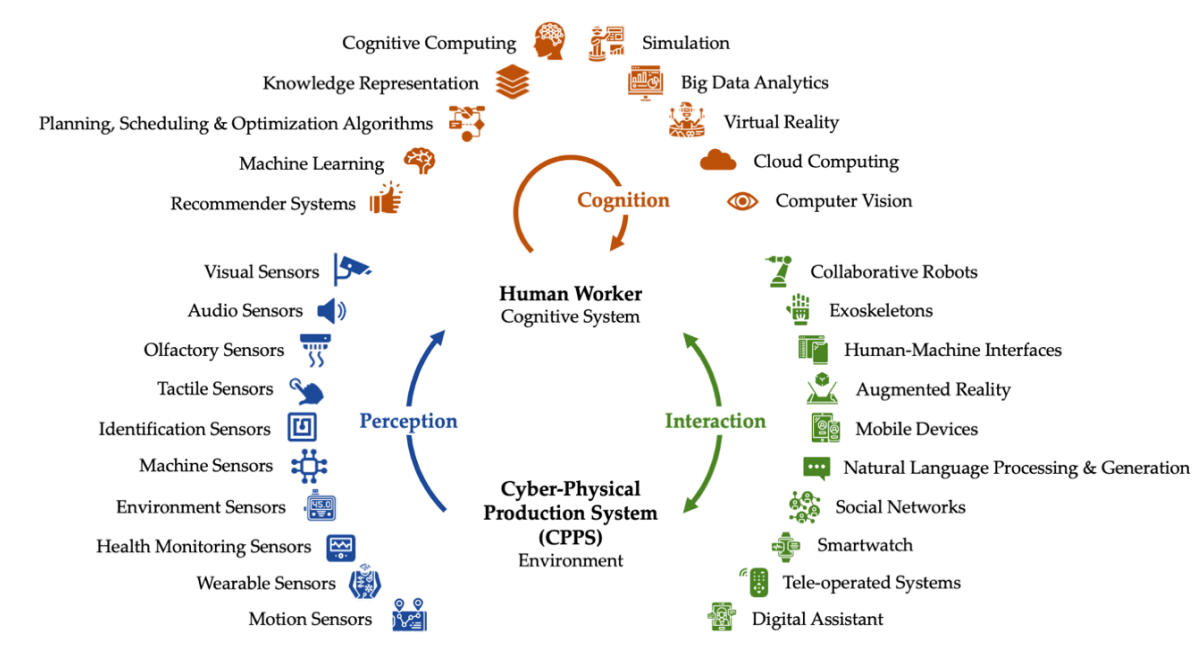
\includegraphics[width=0.8\linewidth]{ThesisFigs/Lando.png}
    \caption{Symbiotic human-machine relationship in Industry 5.0 \cite{Longo2020}}
    \label{figure:Ov4}
\end{figure}

In order to better integrate humans in CPS, the concept of Human Digital Twins is finding increasing popularity, in order to better monitor, evaluate and optimize human performance, ergonomics and well-being \cite{Locklin2021}. Development of Human Digital Twins involves the deployment of a model of humans using sensor data which provides insight into their behavior and attributes, which may include their physical, physiological, cognitive, and emotional states \cite{Miller2022}. Creating a symbiotic human-robot collaboration system requires the use of dynamic monitoring of humans and resources using smart sensors, active collision avoidance, dynamic planning, and context-aware adaptive robot control \cite{Wang2019}.

\section{Human Intent and Motion Prediction}
A truly effective Human-Centric Digital Twin (HCDT) must go beyond simply monitoring the current state of a human operator; it must be able to anticipate their future actions. This predictive capability is paramount for robots to transition from reactive assistance to proactive, intelligent collaboration \cite{Asad_Intention_2025}. The endeavor to create such proactive robotic assistants draws upon several interconnected research areas, including human intent prediction, AI-driven motion generation, and the application of Large Language Models (LLMs) to robotics.

\subsection{Human Intent Prediction for Collaborative Environments}
Anticipating human intent is pivotal to enhancing safety, ergonomics, and effective collaboration in Industry 5.0. Early work often focused on trajectory prediction in constrained scenarios \cite{Huang2021}. More recent approaches have sought to infer higher-level goals. For instance, Huang et al. \cite{Huang2022} proposed a hierarchical intention-tracking framework for assembly tasks, utilizing OpenPose and Kalman filtering to track wrist positions and infer both high-level task goals and low-level current actions. Similarly, Mangin et al. \cite{Mangin2022} developed hierarchical planners that infer human goals using partially observable Markov decision processes for procedural tasks. The use of egocentric data has also gained traction, with works like Mascaro et al. \cite{Mascaro2022} developing intention-conditioned hierarchical architectures for long-term action anticipation. However, many existing methods focus on recognizing intent from past actions rather than proactively forecasting future motion linked to that intent.

\subsection{AI-Driven Virtual Human Motion Generation}
Generating realistic and controllable human motion is a long-standing challenge. The field has historically relied on motion capture (MoCap) datasets, which provide high-fidelity kinematic data. A significant advancement was the creation of large-scale datasets pairing MoCap data with natural language descriptions, such as HumanML3D \cite{Guo_2022_CVPR}. With the advent of kinematic diffusion models, the Human Motion Diffusion Model (MDM) \cite{tevet2023human} demonstrated a remarkable ability to generate complex motions from text prompts alone. However, these purely kinematic approaches often produce physically implausible motions. To address this, PhysDiff \cite{Yuan2023} introduced a novel physics-guided approach that incorporates a physics simulator directly into the diffusion process, thereby correcting the motion to adhere to physical constraints. These MoCap-based methods, however, often lack the rich scene-interaction context necessary for robustly forecasting actions in unstructured, real-world environments.

\subsection{The Role of LLMs in Intelligent Robots}
The advent of LLMs has opened new avenues for enhancing the semantic understanding and planning capabilities of robotic systems. LLMs can parse natural language instructions, reason about task goals, and even generate plans or code snippets for robotic execution \cite{Fan2024, Singh2023}. For instance, SayCan \cite{Ahn2022} demonstrated how LLMs can propose high-level actions grounded by pretrained robotic skills. Singh et al. \cite{Singh2023} developed ProgPrompt using programmatic LLM prompts to generate executable plans. These works highlight LLMs' potential in interpreting complex instructions and decomposing them into actionable steps, a critical component for understanding human intent. However, grounding LLM outputs in the physical world and integrating them with continuous motion generation remain active research areas.

\section{Enabling Technologies}
A number of technical challenges exist in the implementation of HCDTs. This paper discusses the key technologies which can be used for the development of HCDTs, focusing on sensing technologies, computational intelligence, simulation, and visualization tools. A generic framework incorporating these technologies is presented in Figure \ref{figure:framework1}.

\begin{figure}[h]
    \centering
    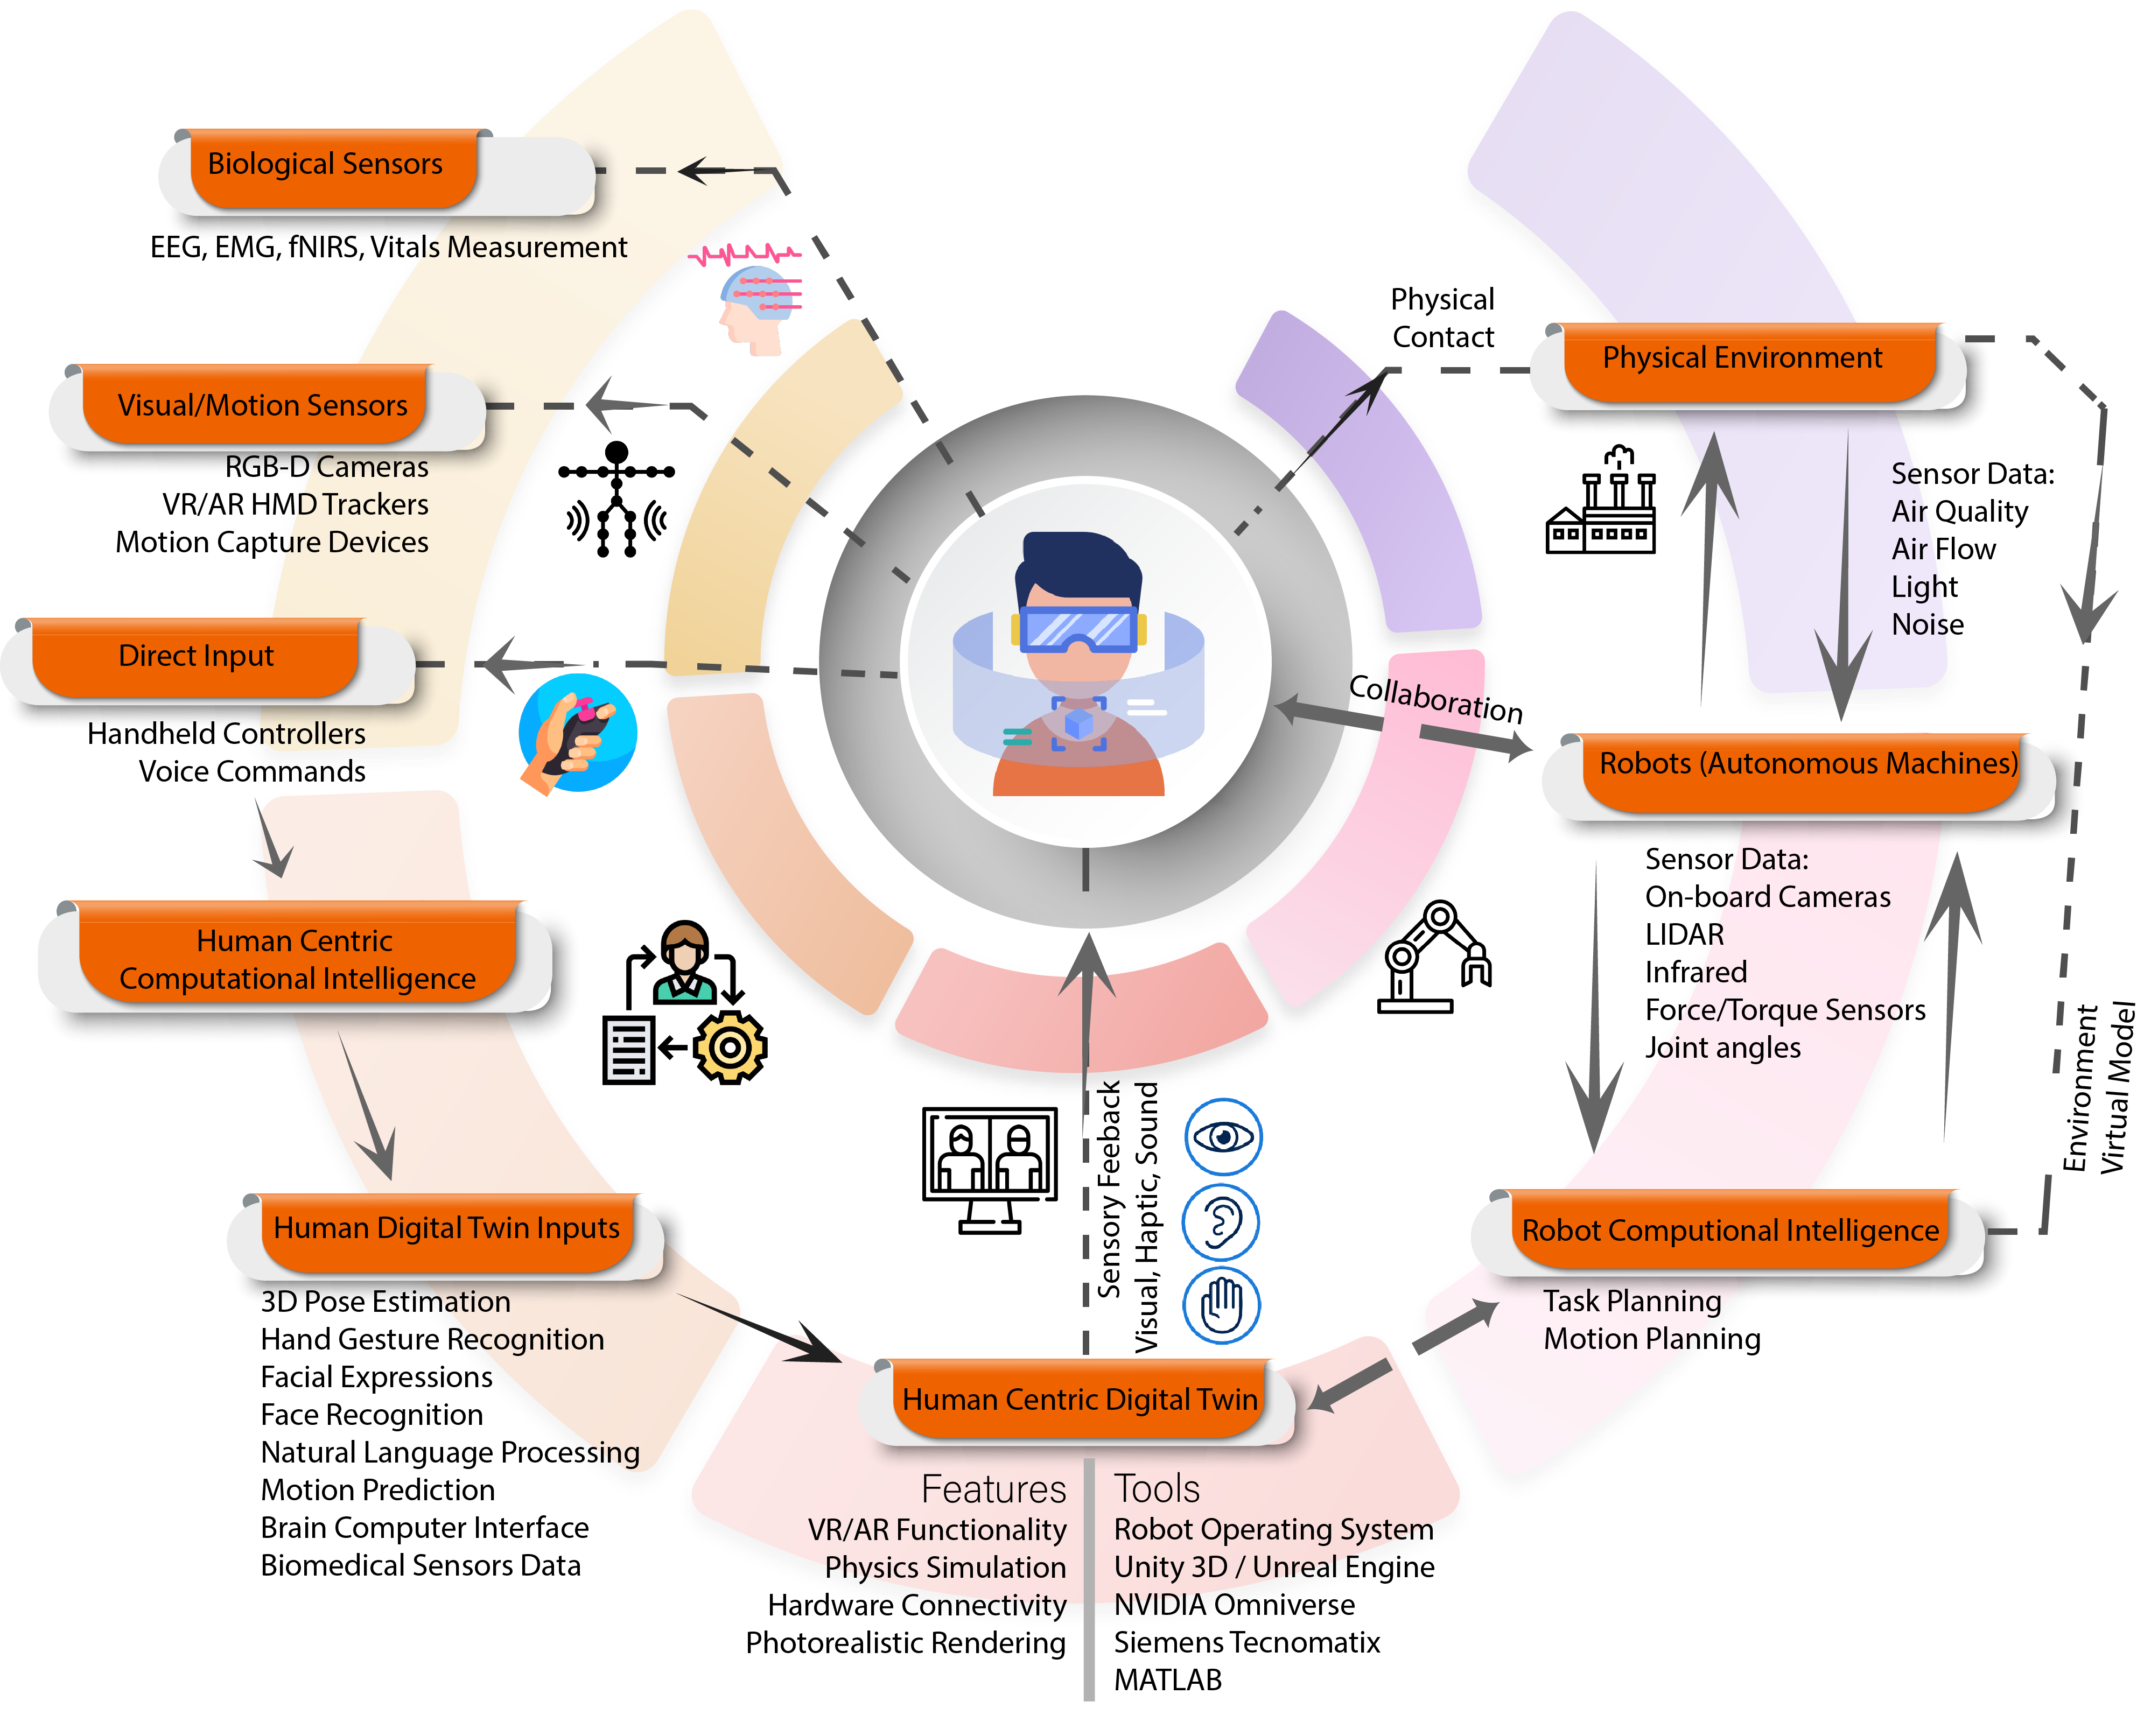
\includegraphics[width=1\linewidth]{ThesisFigs/Framework.png}
    \caption{Enabling Technologies and framework of Human-Centric Digital Twins in Industry 5.0}
    \label{figure:framework1}
\end{figure}

\subsection{Human-focused Sensors}
To create HCDT-driven CPS, sensors are deployed to collect digital data from humans. For accurate human skeletal tracking and joint monitoring, optical and non-optical sensing devices are used. Optical marker-based devices, such as Optitrack and VICON are widely used. On the other hand, optical marker-less technology and video-based human motion tracking devices including RGB-D Cameras \cite{Yi2022, Dimitropoulos2021} and Kinect \cite{Khatib2021, Liu2021} are also extensively used. Non-optical tracking devices include wearable inertial measurement units (IMUs) \cite{Yi2021}.

Different Biological sensors are also being used to measure the physiological data of humans to monitor human behavior during human-robot collaboration \cite{bs1-Tiberio}. Physiological sensors, such as Electroencephalogram (EEG) \cite{bs4-bi} and EMG \cite{bs6-yeom}, capture signals generated from the human body and can infer important information, such as the intention of human operators \cite{bs5-hakonen}.

\subsection{Computational Intelligence}
Artificial Intelligence and Machine Learning are central to realizing the promise of HCDTs.

\subsubsection{Computer Vision}
Creating a high-fidelity Human Digital Twin may involve recognition of human facial features, expression, pose, and gestures. Deep Neural Networks and Computer Vision are being used extensively for this purpose. Yi et al. \cite{Yi2022} uses RGB-D Sensors for posture estimation using a Convolutional Neural Network (CNN). Machine Learning based computer vision has been widely used in literature for safe Human-Robot Collaboration \cite{Droder2018, Osama2019}.

\subsubsection{Classification Methods}
Supervised Learning based classification techniques such as CNNs, Long Short-term Memory (LSTMs), and Hidden Markov Models (HMM) have been used for motion and intent detection and prediction in HRC \cite{Zhang2022-Fusion, AI-MP-Manu, AI-DT-Survey}.

\subsubsection{Reinforcement Learning}
In Reinforcement Learning (RL) algorithms, agents learn their control policy through unsupervised learning. Deep Reinforcement techniques leverage deep neural networks in combination with RL algorithms, such as Q-Learning to solve complex problems. Reinforcement learning has found widespread use in motion planning \cite{Liu2022, Vrabic2021}, and in decision-making in human-centric applications \cite{Sun2022, Xia2021, Matulis2021}.

\subsection{Simulation Tools}
For the development of a DT, different simulation tools are required to create an interaction between physical objects and their virtual twins.

\subsubsection{Numerical Analysis Tools}
Finite Element Analysis (FEA) is often necessary for Multiphysics simulations of physical assets. FEA tools, such as ANSYS \cite{Aubert2021}, COMSOL \cite{Zhu2022} and ABAQUS \cite{Liang2018}, have been frequently used to create DTs for biomedical applications and physical assets for which health/condition monitoring is desired \cite{Aivaliotis2019}.

\subsubsection{Robotics Simulation Tools}
Robotics simulators allow developers to design, test, and evaluate robotic systems in virtual environments. Gazebo is one of the most commonly used simulators \cite{Thumm2022, Bansal2019, Vrabic2021}. It is an open-source simulator that can be integrated with the Robot Operating System (ROS), one of the most widely used platforms by robotics researchers \cite{Macenski2022}.

\subsubsection{Game Physics Engines}
Game development applications and Physics engines are valuable tools for the development and simulation of DTs \cite{Clausen2022}. The most commonly used physics engine is NVIDIA's PhysX, which is used by Unity and Unreal Engine. In recent years, these have widely been used in the development of DTs \cite{BioMech-Eval, Mania2020, Yun2022, Mourtzis2022-MR}.

\subsection{Data Visualization and Interaction}
\subsubsection{Photorealistic Rendering}
The creation of virtual models in DTs begins with 3D modeling tools like Blender \cite{Alexopoulos2020} or 3ds Max \cite{Wu2019}. The ability of these tools to create photorealistic rendered images can be used to generate training data for ML algorithms and to provide a realistic user experience. Often, models are exported to platforms such as NVIDIA Omniverse \cite{Akar2022}, Unity \cite{Dianatfar2021} or Unreal Engine \cite{Mania2020}.

\subsubsection{Immersive User Experience}
The use of DTs creates opportunities for a rich immersive user experience through Virtual Reality, Augmented Reality, and Mixed Reality. In Augmented Reality, virtual objects are superimposed on real images, using a Head Mounted Display (HMD) such as Microsoft Hololens \cite{Kunz2022, Li2022}. Mixed Reality (MR) allows for co-existence and interactivity between the physical and the virtual environment \cite{Ke2019}, which can be used for intuitive teleoperation of robotic manipulators \cite{Su2022}.

\section{Challenges in Deformable Object Manipulation}
Manipulation of deformable materials is a good example of Moravec’s paradox, which states that what is easy for humans tends to be challenging for robots. Human workers frequently perform such manipulation tasks in maintenance, assembly, and manufacturing settings, handling a variety of materials including flexible hoses, cables, textiles, and composite reinforcements. Collaborative robotics and automation have faced persistent challenges in adopting these tasks due to the high dimensionality of deformable materials, which complicates the extraction and representation of their state. Furthermore, there exists a significant sim-to-real gap caused by the challenge of creating high-fidelity simulation and learning environments.

\subsection{Deformable Object Modeling}
Physics-based simulation of deformable materials often relies on geometric representations using particles or meshes. For a thorough review of the foundational aspects of models and dynamics of deformable materials, see \cite{ModelDeformReview}. One of the most promising methods is Position Based Dynamics (PBD) \cite{PBD}. In PBD, objects are represented by a set of vertices and constraints. The simulation predicts new positions for the vertices and then adjusts these positions through an iterative solver to satisfy the constraints. This approach is computationally efficient and robust, making it suitable for real-time applications.

\subsection{Differentiable Simulation and Learning}
Differentiable physics engines have revolutionized robotic manipulation by enabling gradient-based optimization of complex interactions. \cite{Li2023} and \cite{Lin2022} demonstrated how differentiable simulation accelerates skill acquisition for deformable objects. \cite{Liu2023} extended this to cloth manipulation, coupling articulated rigid bodies with deformable models. Complementary to simulation, \cite{Chi2022} introduced iterative residual policies for goal-conditioned manipulation, while \cite{Salhotra2022} leveraged imitation learning to transfer human expertise to robots. These approaches highlight the synergy between simulation fidelity and data-driven learning.

\section{Application Domains}
Digital Twin Technology has recently been applied in a range of industries. Here, we emphasize key application domains where human-centricity is of paramount importance.

\subsection{Ergonomics and Safety}
In Smart Factories, as humans and collaborative robots begin to share workspaces, it is necessary to ensure human safety and optimize ergonomics. Havard et al. \cite{Havard2019} created a DT to carry out a Safety and Ergonomics assessment in VR. In HRC safety, collision avoidance is an important challenge. Liu et al. \cite{Liu2021} employs a deep reinforcement learning algorithm to allow a Cobot to reach a target state while minimizing the risk of collision with a human hand. A generic layout for HCDTs for ergonomics and safety is shown in Figure \ref{figure:FrameworkSafety}.

\begin{figure}[h]
    \centering
    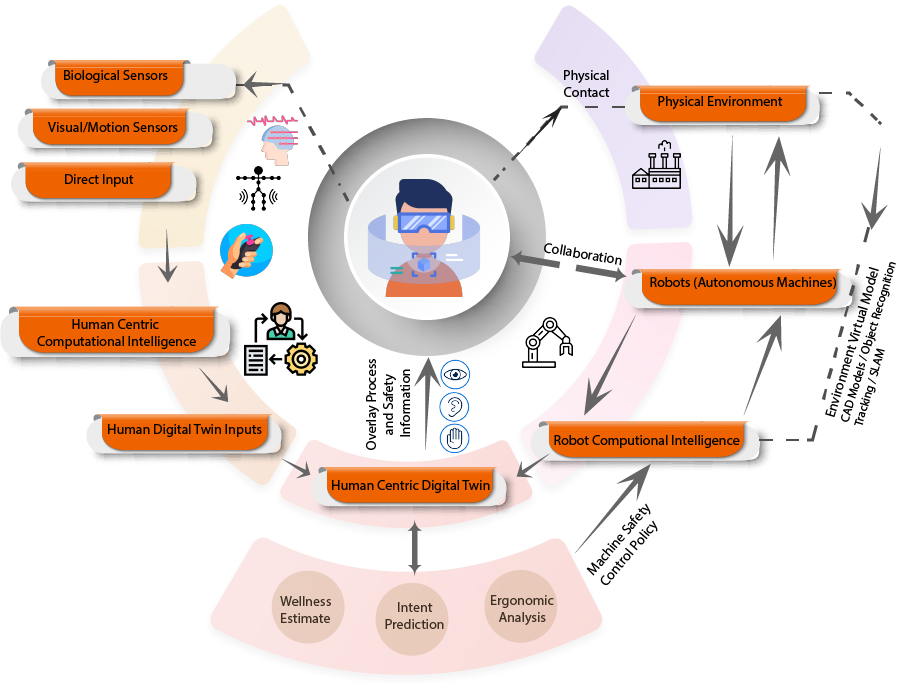
\includegraphics[width=1\linewidth]{ThesisFigs/FrameworkSafety.png}
    \caption{Generic framework for HCDT for safety and ergonomics}
    \label{figure:FrameworkSafety}
\end{figure}

\subsection{Training and Testing of Robotics Systems}
DTs have found great utility in the training and testing of Robotics Systems. DTs can provide a high-fidelity virtual environment to generate a vast amount of test data to viably train an ML model and transfer it to the physical robot. NVIDIA has demonstrated this capability using its platform NVIDIA Omniverse to create DTs of warehouses for training of AI models \cite{omniverse}. Mania et al. employed photorealistic simulations rendered in a game engine to increase the performance of the perception system of a mobile robot \cite{Mania2020}. A generic framework for using HCDTs for training robotics systems is shown in Figure \ref{figure:FrameworkML}.

\begin{figure}[h]
    \centering
    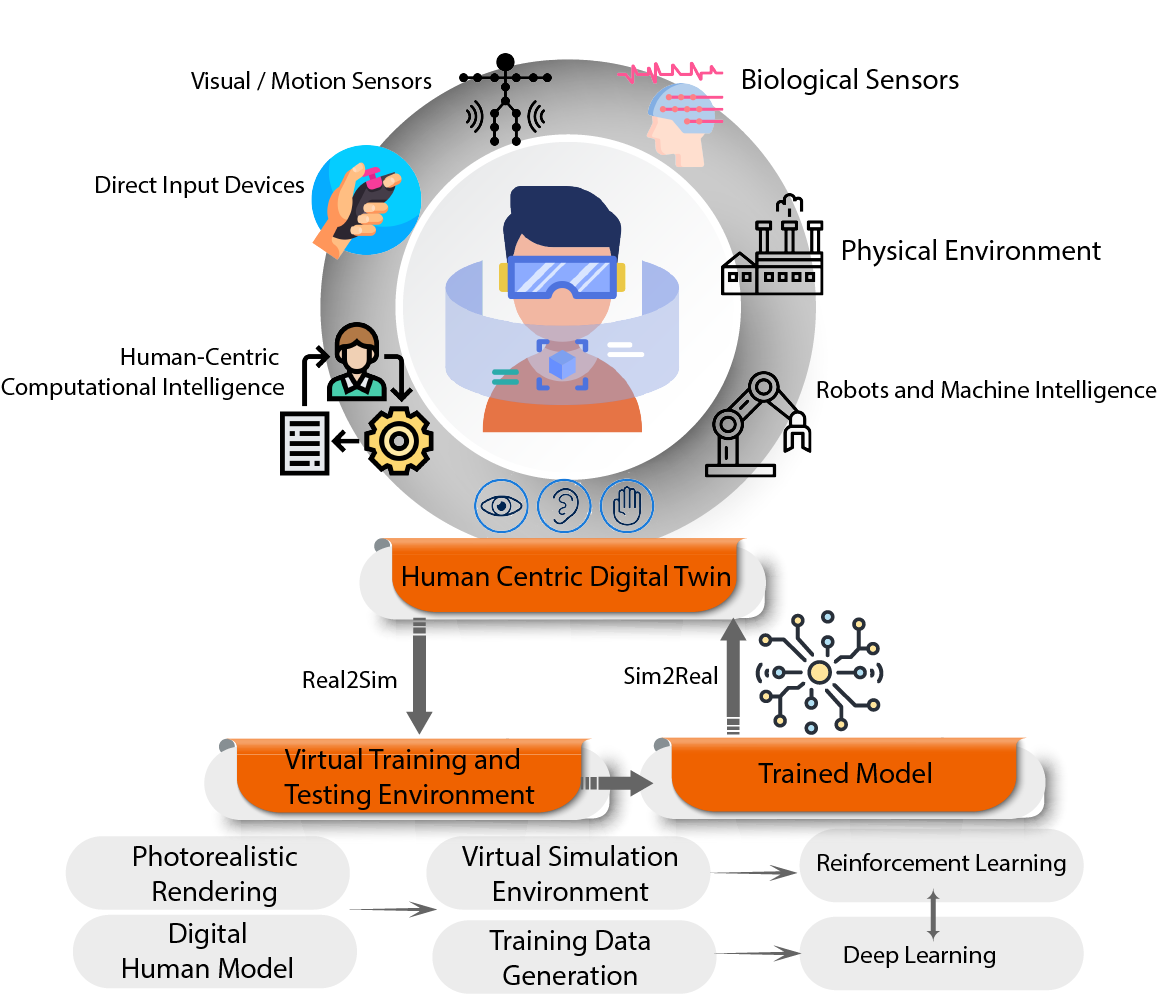
\includegraphics[width=1\linewidth]{ThesisFigs/TrainingFrameworkReduced2.png}
    \caption{Generic framework for Robotics System Training}
    \label{figure:FrameworkML}
\end{figure}

\subsection{User Training and Education}
VR/AR technologies are already widely used in training and teaching. The use of AR/VR headsets enable operators to get a better understanding of a process, for remote assistance and operator training \cite{Perno2022}. DTs have also been used in enhanced surgical training, where the use of DTs with haptic feedback is reported to increase accuracy and reduce cognitive load on surgeons \cite{Hagmann2021}.

\subsection{Product and Process Design, Validation and Testing}
The prospect of using DTs in combination with immersive technologies can be utilized to enhance and enrich the process and product design. Malik et al. \cite{Malik2019-Tariq} leveraged DTs and virtual reality for HRC design and planning. The proposed architecture uses bi-directional information sharing between the physical and virtual robot and human operator. In the VR environment, designers can manipulate objects and study the HRC design from the perspective of visibility, reach, and ergonomics to optimize cycle times and safety.

\subsection{Security of Cyber-Physical systems}
Security and reliability are important issues in DTs, more so in HCDTs. In the context of a Collaborative Robotic Cyber-Physical System (CRCPS), Khalid et al. present a framework for secure CRCPS based on authentication and data integrity checks \cite{Khalid2018}. Digital Twins can themselves be used for enhancing security: Deitz et al. sets out formal requirements of a security framework that employs DT simulations to detect, analyze and handle security incidents \cite{Dietz2020}.

\subsection{Rehabilitation, Well-being and Health Management}
In the medical domain, Human Digital Twin technology has found more maturity and acceptance. Medical Digital Twins (MDTs) have been used in many areas including pulmonology \cite{Zhang2021} and orthopedics \cite{Hernigou2021}. MDTs may involve using clinical imaging techniques to develop Patient-specific solutions, for example for the human tongue \cite{Calka2021}, tibia \cite{Aubert2021}, or aortic walls \cite{Liang2018}. Figure \ref{figure:MedicalFramework} illustrates a generic layout for healthcare applications.

\begin{figure}[h]
    \centering
    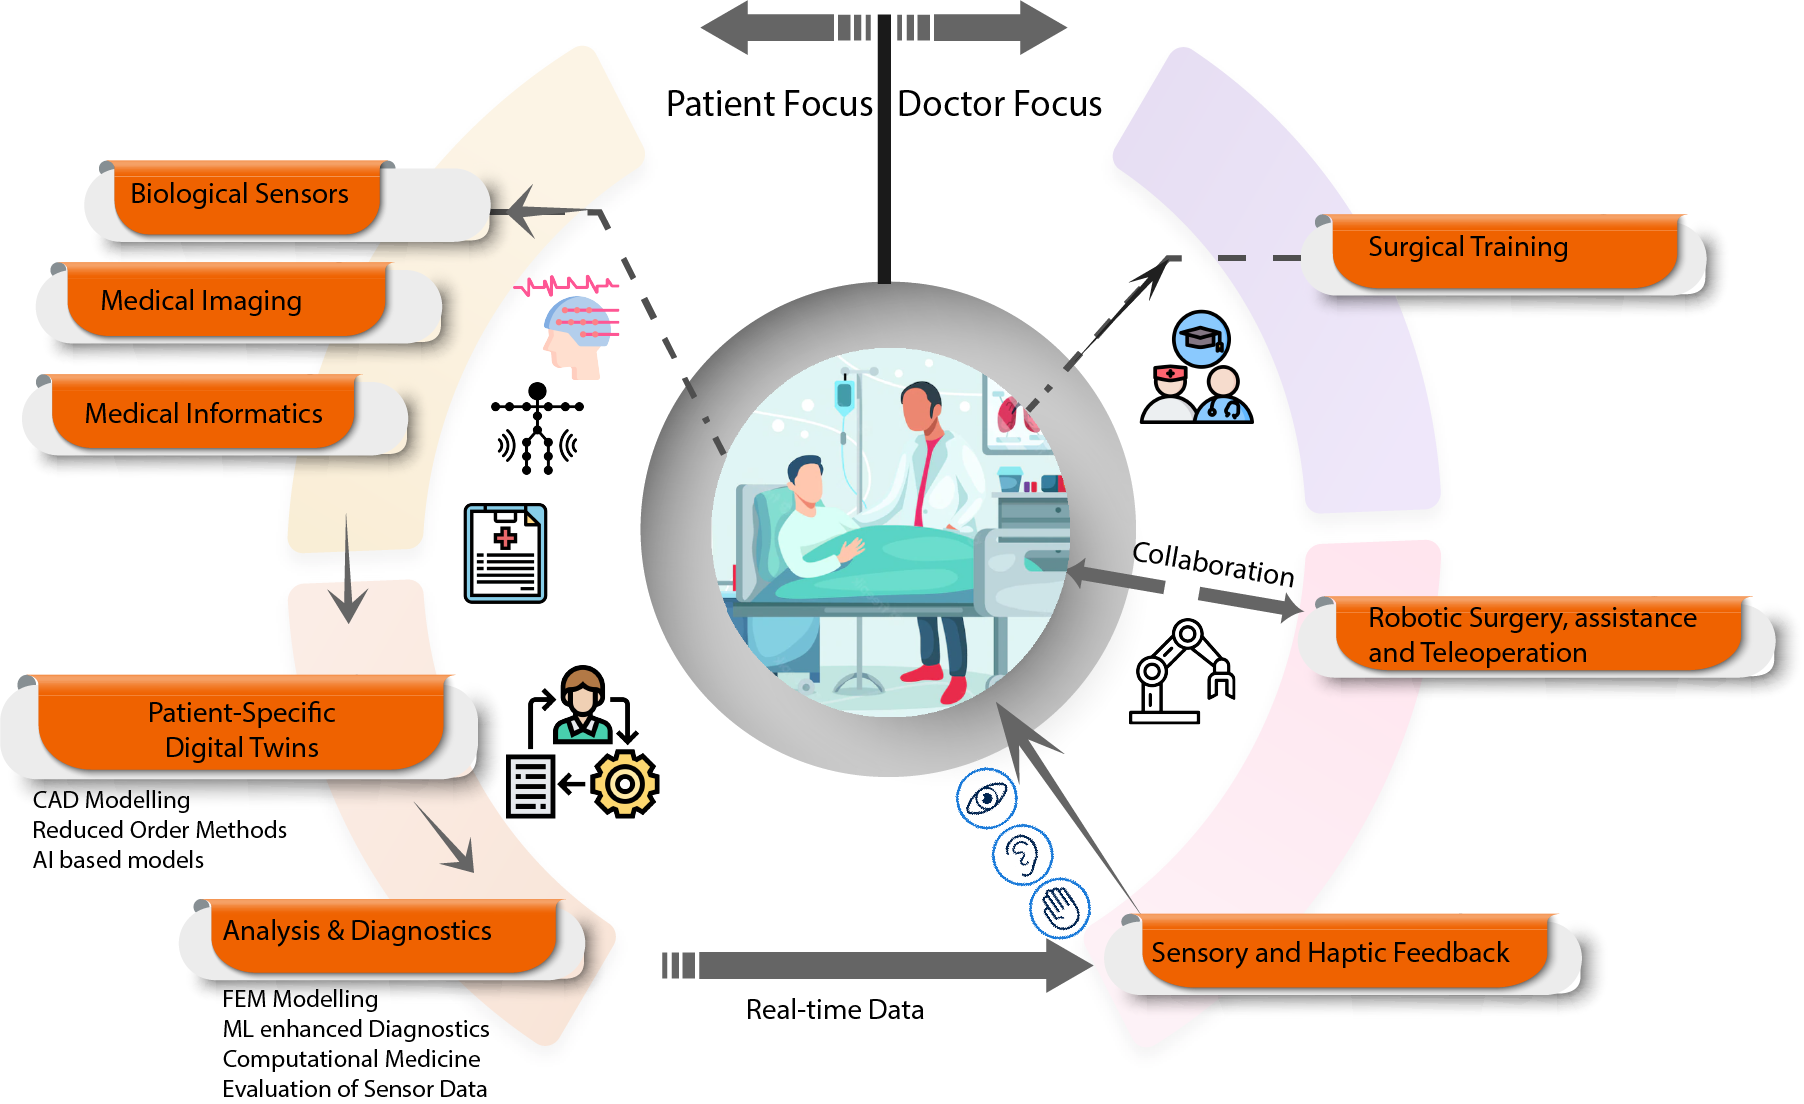
\includegraphics[width=0.9\linewidth]{ThesisFigs/MedicalFramework.png}
    \caption{Generic framework for DTs in healthcare}
    \label{figure:MedicalFramework}
\end{figure}

\section{Research Gap}
This chapter has provided a comprehensive review of Human-Centric Digital Twins, their enabling technologies, and key application domains. A key shortcoming observed from current DT literature is that the focus is almost entirely on the physical assets of a CPS, and not on human operators. To address this, a deeper understanding of human intent and motion is required, especially for complex tasks such as the manipulation of deformable objects. The enabling technologies for this purpose, such as AI-driven algorithms for object recognition and collision avoidance, have reached some degree of maturity. However, there is a lack of literature in which all these enabling technologies are utilized together in a synergistic manner to enhance human-machine interaction in industrial settings. The following chapters will detail a novel framework designed to bridge this gap, with a specific focus on developing proactive robotic assistance for composites manufacturing.
